\chapter{Elaborazione di immagini lunari} \label{chap:techniques}

Questo capitolo si propone di approfondire le tecniche di elaborazione delle immagini lunari, illustrando le nozioni teoriche alla base degli algoritmi implementati nel progetto. Ogni tecnica verrà descritta in dettaglio, partendo da calibrazione e allineamento, passando per pre-processing e stacking, per concludere con il post-processing. Quando necessario, verranno forniti pseudocodice e descrizioni dei processi matematici applicati alle immagini; l'implementazione sarà invece discussa nel capitolo \ref{chap:implementation}.

\section{Calibrazione di immagini} \label{sec:calibration}

La \textbf{calibrazione} delle immagini è un passaggio fondamentale nell'astrofotografia, necessario per rimuovere rumore e artefatti introdotti dalla strumentazione. In particolare, nel contesto delle immagini lunari, la calibrazione è utile per rimuovere il rumore termico e i difetti del sensore, oltre a uniformare l'illuminazione dell'immagine. Questo processo è composto da tre fasi principali: la cattura di \textit{bias frames}, \textit{dark frames} e \textit{flat frames}. Tali scatti devono essere acquisiti con la fotocamera nello stesso stato in cui sono state scattate le immagini lunari, in particolare nelle stesse condizioni termiche. Infatti, quando viene eseguita una sessione di molti scatti, o con lunghe esposizioni, la macchinetta tende a scaldarsi causando effetti non sempre trascurabili, e sono proprio quelli che vogliamo mitigare mediante la fase di calibrazione. In questa fase gli scatti della luna vengono denominati \textit{light frames}  \cite{calibration}.

\subsection{Bias Frames} \label{subsec:bias}

I \textbf{bias frames} son scatti acquisiti con il tempo di esposizione più breve possibile (il minimo supportato dalla macchina fotografica, idealmente zero), ISO uguale a quello dei light frames e con l'otturatore della fotocamera chiuso. Questi frame catturano il \textbf{rumore di bias}, un segnale di offset introdotto dall'elettronica del sensore in assenza di luce. Il rumore di bias è presente in tutte le immagini acquisite con una macchina fotografica, e varia leggermente da pixel a pixel.

Per correggere questo rumore si calcola il cosiddetto \textbf{master bias} combinando i diversi bias frames, generalmente calcolandone la media. Il master bias viene poi sottratto da tutte le immagini acquisite, inclusi gli altri frame di calibrazione.

\begin{algorithm}[H]
    \caption{\texttt{- Calcolo del master bias}:\\ Data la lista di bias frames $B_f$, l'algoritmo calcola il master bias $M_b$} \label{alg:bias}
    \begin{algorithmic}[1]
        \Function{calculate\_master\_bias}{$B_f$}
            \State $N \gets$ \text{numero di bias frames}
            \State $M_b \gets 0$
            \For{$i \gets 1$ to $N$}
                \State $M_b \gets M_b + \dfrac{B_f[i]}N$ \Comment{Media dei bias frames}
            \EndFor
            \State \textbf{return} $M_b$
        \EndFunction
    \end{algorithmic}
\end{algorithm}

\textbf{Applicazione:} Per applicare il master bias a un'immagine, si sottrae semplicemente il master bias dall'immagine originale. In formula, data un'immagine \textit{original} e il master bias \textit{master\_bias}, l'immagine calibrata \textit{final\_image} sarà data da:

$$
    final\_image = original - master\_bias
$$

\subsection{Dark Frames} \label{subsec:dark}

I \textbf{dark frames}, acquisiti con stessi ISO e tempi di cattura dei light frames, ma con l'otturatore chiuso, catturano il \textbf{rumore termico} causato dall'agitazione termica degli elettroni nel sensore. Questo rumore aumenta con il tempo di esposizione e con la temperatura del sensore e può variare significativamente tra scatti differenti.

Per correggere il rumore termico, si calcola il \textbf{master dark} combinando i diversi dark frames, generalmente calcolandone la media. Il master dark viene poi sottratto ai light frames e ai flat fames. È importante sottrarre il master bias dai dark frames prima di calcolare il master dark, per evitare di sommare due volte il rumore di bias.

\begin{algorithm}[H]
    \caption{\texttt{- Calcolo del Master Dark}:\\ Data la lista di dark frames $D_f$ e il master bias $M_b$, l'algoritmo calcola il master dark $M_d$.} \label{alg:dark}
    \begin{algorithmic}[1]
        \Function{calculate\_master\_dark}{$D_f$, $M_b$}
            \State $N \gets$ \text{numero di dark frames}
            \State $M_d \gets 0$
            \For{$i \gets 1$ to $N$}     
                \State $ D_c \gets D_f[i] - M_b$ \Comment rimozione del bias
                \State $M_d \gets M_d + \dfrac {D_c} N$ \Comment media dei dark frames
            \EndFor
            \State \textbf{return} $M_d$
        \EndFunction
    \end{algorithmic}
\end{algorithm}

\textbf{Applicazione:} Per applicare il master dark a un'immagine, si sottrae semplicemente il master dark dall'immagine originale. In formula, data un'immagine \textit{original} e il master dark \textit{master\_dark}, l'immagine calibrata \textit{final\_image} sarà data da:

$$
    final\_image = original - master\_dark
$$

\subsection{Flat Frames} \label{subsec:flat}

I \textbf{flat frames} sono scatti acquisiti fotografando una sorgente di luce uniforme, come un cielo crepuscolare o un pannello luminoso. Vengono acquisiti con lo stesso tempo di esposizione e ISO dei light frames, ma con l'otturatore aperto. Questi frame catturano le variazioni nella risposta dei pixel del sensore e il \textbf{rumoe di vignettatura} introdotto dal sistema ottico, ovvero la diminuzione dell'illuminazione verso i bordi dell'immagine.

Per correggere queste imperfezioni si calcula un \textbf{master flat} combinando i diversi flat frames, solitamente attraverso la media. Prima di calcolare il master flat, è necessario sottrarre sia il master bias che il master dark dai flat frames. Una volta calcolato il master flat, questo viene normalizzato dividendolo per il valore medio dei suoi pixel. Il master flat viene poi utilizzato per normalizzare le immagini scientifiche, dividendo ogni pixel dell'immagine per il corrispondente valore nel master flat.

\begin{algorithm}[H]
    \caption{\texttt{- Calcolo del Master Flat}:\\ Data la lista di flat frames $F_f$, il master bias $M_b$ e il master dark $M_d$, l'algoritmo calcola il master flat normalizzato $M_f$.} \label{alg:flat}
    \begin{algorithmic}[1]
        \Function{calculate\_master\_flat}{$F_f$, $M_b$, $M_d$}
            \State $N \gets$ \text{numero di flat frames}
            \State $M_f \gets 0$
            \For{$i \gets 1$ to $N$}
                \State $F_c \gets F_f[i] - M_b - M_d$ \Comment{rimozione di bias e dark}
                \State $M_f \gets M_f + \dfrac {F_c} N$ \Comment{media dei flat frames}
            \EndFor
            \State $M_f \gets \dfrac {M_f} {\text{mean}(M_f)}$ \Comment{normalizzazione}
            \State \textbf{return} $M_f$
        \EndFunction
    \end{algorithmic}
\end{algorithm}

\textbf{Applicazione:} Per applicare il master flat a un'immagine, si divide semplicemente l'immagine originale:

$$
    final\_image = \dfrac {original} {M_f}
$$

Nel contesto di questo progetto, i flat frames non sono stati acquisiti per due principali motivi. In primo luogo, la loro acquisizione risulta complessa e richiede condizioni specifiche che non sono state facilmente riproducibili durante le sessioni fotografiche. In secondo luogo, l'effetto della vignettatura non ha rappresentato un problema significativo nelle immagini ottenute, poiché la Luna era posizionata verso il centro degli scatti e occupava meno di un terzo dell'altezza dell'immagine. Nonostante ciò, il processo di calibrazione è stato comunque implementato per consentire l'utilizzo di flat frames, garantendo flessibilità e scalabilità del metodo di elaborazione adottato.

\subsection{Processo completo di calibrazione} \label{subsec:calibration_process}

Il processo completo di calibrazione applica in sequenza le correzioni con i master frames; si sottraggono master bias e master dark e si divide per il master flat:

\begin{algorithm}[H]
    \caption{\texttt{- Calibrazione di un'immagine}:\\ Data un'immagine $Img$ e i master frames $M_b$, $M_d$ e $M_f$, l'algoritmo calcola l'immagine calibrata $Out$.} \label{alg:calibration}
    \begin{algorithmic}[1]
        \Function{calibrate\_image}{$Img, M_b, M_d, M_f$}
            \State $Out \gets \dfrac {Img - M_b - M_d} {M_f}$
            \State \textbf{return} $Out$
        \EndFunction
    \end{algorithmic}
\end{algorithm}

\textbf{Applicazione:} Per calibrare un'immagine, si applica la funzione \textit{calibrate\_image} con i master frames calcolati. In formula, data un'immagine \textit{original} e i master frames $M_b$, $M_d$ e $M_f$, l'immagine calibrata \textit{final\_image} sarà data da:

$$
    final\_image = \dfrac {original - M_b - M_d} {M_f}
$$

Questo processo (illustrato in figura \ref{fig:calibration})  permette di ottenere immagini corrette da rumori elettronici, termici e da imperfezioni ottiche.

\begin{figure} [H]
    \centering
    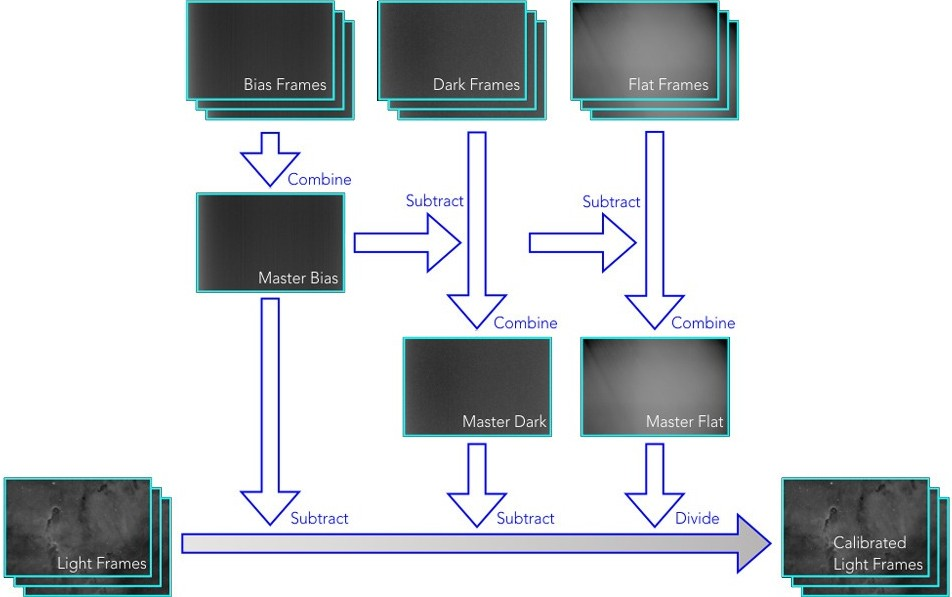
\includegraphics[scale = 0.45]{../assets/calibration_procedure.jpg}
    \captionsetup{justification=centering}
    \caption{Illustrazione schematica dell'uso di immagini di calibrazione \cite{calibration_img}} \label{fig:calibration}
\end{figure}

\section{Allineamento delle immagini} \label{sec:alignment}

L'allineamento delle immagini è un passaggio cruciale nell'elaborazione delle immagini lunari, necessario per compensare eventuali spostamenti o rotazioni tra gli scatti e per combinare efficacemente più immagini tramite tecniche di \textit{stacking}. Questo processo si basa sull'identificazione di punti caratteristici comuni tra le immagini e sul calcolo delle trasformazioni geometriche necessarie (nel nostro caso \hyperref[subsec:homography]{trasformazioni omografiche}) per sovrapporle perfettamente. L'allineamento delle immagini può essere eseguito manualmente, ma è preferibile utilizzare algoritmi automatici per garantire una maggiore precisione e riproducibilità.

\subsection{Feature Detection e Matching ORB, SIFT e SURF} \label{subsec:feature_detection}

Gli algoritmi di \textit{feature detection} e \textit{matching} individuano punti di interesse nei distintivi nelle immagini, come bordi, angoli o altre caratteristiche uniche, e calcolando descrittori che rappresentano l'intensità locale attorno a ciascun punto. Successivamente, i descrittori vengono confrontati per trovare corrispondenze tra i punti di interesse delle diverse immagini, consentendo di determinare le trasformazioni geometriche necessarie per allineare le immagini.

Tra i vari algoritmi di feature detection e matching disponibili, tre si distinguono per la loro efficacia e diffusione: ORB (Oriented FAST and Rotated BRIEF), SIFT (Scale-Invariant Feature Transform) e SURF (Speeded-Up Robust Features), i quali sono in grado di identificare punti di interesse invarianti rispetto a rotazioni, traslazioni e scalature, e sono particolarmente adatti per l'allineamento di immagini astronomiche.

\begin{itemize}
    \item \textbf{SIFT} (Scale-Invariant Feature Transform): è noto per la sua elevata accuratezza e robustezza a cambiamenti di scala, rotazione e illuminazione. L'algoritmo identifica i keypoints costruendo una piramide di immagini a diverse scale e cercando i massimi locali. L'orientamento di ogni keypoint viene determinato analizzando gli istogrammi dell'orientamento del gradiente nell'intorno del punto stesso. Un descrittore SIFT ha generalmente 128 dimensioni e viene calcolato campionando gli orientamenti del gradiente in una griglia 16x16 attorno al punto chiave. Questo algoritmo è molto preciso, ma anche computazionalmente costoso, il che può essere problematico per applicazioni in tempo reale o con grandi volumi di dati \cite{sift}.
    
    \item \textbf{SURF} (Speeded-Up Robust Features): è stato sviluppato come alternativa più veloce a SIFT. Utilizza un'approssimazione del determinante dell'Hessiana per il rilevamento di keypoints e un descrittore basato sulla somma delle risposte alle wavelet di Haar. Questo approccio rende SURF più efficiente dal punto di vista computazionale rispetto a SIFT, pur mantenendo un buon livello di accuratezza e robustezza. Inoltre, SURF integra le informazioni sul gradiente all'interno di un sotto-patch, migliorando le performance nella rilevazione di caratteristiche in presenza di rumore. Tuttavia, come SIFT, anche SURF è coperto da brevetti che ne limitano l'utilizzo \cite{surf}.

    \item \textbf{ORB} (Oriented FAST and Rotated BRIEF): è un descrittore binario veloce, progettato per essere efficiente dal punto di vista computazionale e libero da restrizioni di licenza. Combina il rilevatore di keypoints FAST, noto per la sua rapidità, con un descrittore BRIEF ruotato, che è efficiente da calcolare e confrontare. ORB aggiunge un componente di orientamento veloce e accurato a FAST, consentendo di calcolare in modo efficiente le caratteristiche BRIEF orientate. Per migliorare le prestazioni, ORB utilizza un metodo di apprendimento per decorrelare le caratteristiche BRIEF, garantendo invarianza rotazionale. Rispetto ad algoritmi come SIFT e SURF, ORB offre prestazioni comparabili in molte situazioni, pur essendo significativamente più veloce; dimostra una notevole resistenza al rumore gaussiano, anche se, in presenza di forti distorsioni prospettiche, può risultare meno preciso \cite{orb}.
 
\end{itemize}

Nel contestro di questo progetto, è stato scelto di utilizzare l'algoritmo ORB grazie alla sua efficienza computazionale e alla sua robustezza nei confronti di rotazioni e traslazioni, comuni nelle immagini acquisite senza montature motorizzate. Tuttavia l'implementazione prevede la possibilità di utilizzare anche SIFT e SURF, mediante un'interfaccia comune per la selezione dell'algoritmo di feature detection e matching.

\begin{figure} [H]
    \centering
    \includegraphics[scale = 0.32]{../assets/feature_detection_1.jpg}
    \captionsetup{format=plain}
    \caption{\parbox{0.8\linewidth}{
        Applicazione di ORB (\textbf{a}-\textbf{b}) e RANSAC (\textbf{c}) su due scatti da me acquisiti. \\ \phantom{m}\textbf{a}-\textbf{b}: visualizzazione di 5000 \textit{keypoint} estratti da due immagini} \\ \phantom{MMmnnnc} \textbf{c}: visualizzazione dei \textit{matches} tra i keypoints delle due immagini
    } \label{fig:orb_img}
\end{figure}

\subsection{Trasformazioni omografiche: RANSAC} \label{subsec:homography}

Una \textbf{omografia} è una trasformazione geometrica che mappa punti da un piano a un altro, mantenendo la collinearità e la connessività dei punti. Nel contesto dell'allineamento delle immagini, l'omografia viene utilizzata per correggere le  differenze di posizione, scala, rotazione e prospettiva tra le immagini.

L'omografia è rappresentata da una matrice $3\times3$ denotata con \textbf{H} che descrive una trasformazione tra due piani proiettivi. La relazione tra un punto nell'immagine di origine $(x, y)$ e il suo corrispondente nell'immagine trasformata $(x', y')$ è data dalla seguente equazione:

$$
\begin{bmatrix} x' \\ y' \\ \omega' \end{bmatrix} = H \cdot \begin{bmatrix} x \\ y \\ \omega \end{bmatrix}
$$

dove $\omega$ e $\omega'$ sono i fattori di scala che consentono di rappresentare le trasformazioni proiettive e le coordinate finali sono ottenute dividendo per $\omega'$:

$$
\begin{bmatrix} x'' \\ y'' \end{bmatrix} = \begin{bmatrix} {x'}/{w'} \\ \dfrac {y'} {w'} \end{bmatrix}
$$

L'omografia può essere calcolata a partire da un set di corrispondenze tra punti nelle due immagini, utilizzando l'algoritmo \textbf{RANSAC} (Random Sample Consensus) per stimare i parametri della matrice H.

$$
H = \begin{bmatrix} h_{11} & h_{12} & h_{13} \\ h_{21} & h_{22} & h_{23} \\ h_{31} & h_{32} & h_{33} \ \end{bmatrix}
$$

L'idea alla base di RANSAC è che gli \textit{inlier} (le corrispondenze corrette) concordano tra loro sulla trasformazione da stimare, mentre gli \textit{outlier} (le corrispondenze errate) non concordano e tendono a essere incoerenti \cite{ransac}. 

\begin{enumerate}
    \item Seleziona casualmente un sottoinsieme minimo di corrispondenze. 
    \item Stima il modello (in questo caso, l'omografia) usando il sottoinsieme selezionato.
    \item Calcola un errore di adattamento per tutte le corrispondenze. 
    \item Determina gli inliers come le corrispondenze con errore inferiore a una soglia.
    \item Se il numero di inlier è superiore a una soglia, ricalcola il modello usando tutti gli inlier e termina. 
    \item Altrimenti, ripete i passaggi precedenti per un numero prefissato di iterazioni. 
\end{enumerate}

RANSAC dipende da due parametri: il \textit{numero di iterazioni} e la \textit{soglia di errore}. Un numero maggiore di iterazioni determina quante volte l'algoritmo estrae campioni casuali. Deve essere sufficientemente grande per garantire una probabilità alta di trovare un modello senza outlier. La soglia di errore definisce il massimo errore accettabile per considerare una corrispondenza come inlier. Esistono altri parametri, uno dei quali è il \textit{numero di corrispondenze} da selezionare per stimare l'omografia, solitamente 4. Qui sotto è riportato un esempio di pseudocodice per il calcolo dell'omografia tramite RANSAC.

\begin{algorithm}[H]
    \caption{\texttt{- Algoritmo RANSAC per la stima dell'omografia}:\\ Dati $matches$, la lista di matches, $k$, il numero massimo di iterazioni, $thr$, la soglia per determinare gli inlier e $n$, il numero di corrispondenze da selezionare per l'omografia, l'algoritmo ritorna la matrice omografica stimata.} \label{alg:ransac}
    \begin{algorithmic}[1]
        \Function{estimate\_homography}{$matches, k, thr$}
            \State $H^* \gets$ \textit{null} \Comment{Miglior omografia stimata}
            \State $score^* \gets 0$ \Comment{Miglior punteggio}
            \For{$i \gets 1$ to $k$}
                \State $R \subseteq matches$ con $|R| = n$ \Comment{Seleziona $n$ corrispondenze casuali}
                \State $H \gets$ Stima l'omografia usando $R$
                \State $score \gets 0$
                \For{$m \in matches$}
                    \If{errore($H$, $m$) $< thr$} \Comment{Errore come distanza euclidea}
                        \State $score \gets score + 1$ \Comment{Conta gli   inlier}
                    \EndIf
                \EndFor
                \If{$score > score^*$} \Comment{Seleziona il modello migliore}
                    \State Aggiorna $H^*$ e $score^*$
                \EndIf
            \EndFor
            \State \textbf{return} $H^*$
        \EndFunction
    \end{algorithmic}
\end{algorithm}

Il numero di iterazioni $k$ necessarie per garantire una certa probabilità di successo $P$ dipende dalla percentuale di inlier attesa $p$ e dal numero minimo di punti $n$ richiesti per stimare il modello \cite{ransac_analysis}:

$$
k = \dfrac{\log(1 - P)}{\log(1 - p^n)}
$$

Ad esempio, se si prevede che l'$80\%$ delle corrispondenze siano inlier ($p=0,8$), si desidera una probabilità di successo del $99\%$ ($P=0,99$) e si utilizzano $n=4$ punti per stimare l'omografia, il numero di iterazioni necessarie è:

$$
k = \dfrac{\log(1 - 0.99)}{\log(1 - 0.8^4)} \approx 17.6
$$

\subsection{Algoritmo di allineamento completo} \label{subsec:alignment_complete}

Per ottenere un allineamento più preciso delle immagini, spesso si applica una fase di pre-elaborazione volta a evidenziare le caratteristiche significative. In particolare, i fotogrammi destinati all’estrazione delle caratteristiche vengono convertiti in scala di grigi e sottoposti a filtri per migliorarne nitidezza e contrasto. È importante sottolineare che queste operazioni vengono eseguite su una copia dei fotogrammi, utilizzata esclusivamente per l’estrazione delle caratteristiche, preservando così i dati originali. In questa sezione, tali operazioni sono sintetizzate nella funzione \texttt{enhance()}, (più nel dettaglio nella \cref{subsec:alignment_impl}). 

L'algoritmo completo per l'allineamento delle immagini, che combina le fasi di estrazione delle caratteristiche, corrispondenza dei descrittori, stima dell'omografia tramite RANSAC e applicazione della trasformazione alle immagini, è illustrato nell'\cref{alg:align}.

\begin{algorithm}[H] \caption{\texttt{Allineamento delle immagini}:\\ Data un insieme di immagini $I$, restituisce l'insieme di immagini allineate $A$} \label{alg:align}
    \begin{algorithmic}[1]
        \Function{align\_images}{$I$}
            \State Seleziona un riferimento $r$ \Comment{Tipicamente la più nitida}
            \State $f \gets$ un algoritmo tra ORB, SIFT, SURF
            \State $k_{r}, d_{r} \gets$ f.calculate\_descriptors($r$) \Comment{Calcola keypoints e descrittori di $r$}
            \For{ogni $i$ in $I$}
                \State $k, d \gets$ f.calculate\_descriptors($i$) \Comment{Calcola keypoints e descrittori di $i$}
                \State $m \gets$ match\_descriptors($d_{r}, d$) \Comment{Trova i match tra i descrittori}
                \State $H \gets$ \small ESTIMATE\_HOMOGRAPHY \normalsize ($k_{r}, k, m$) \Comment{Calcola l'omografia}
                \State $a \gets$ apply\_transformation($i$, $H$) \Comment{Applica l'omografia}
                \State Aggiungi $a$ a $A$
            \EndFor
            \State \textbf{return} $A$
        \EndFunction
    \end{algorithmic}
\end{algorithm}

\section{Pre-processing delle immagini} \label{sec:preprocessing}

Il pre-processing delle immagini è quella fase di elaborazione dei singoli scatti (ormai calibrati e allineati), necessaria per migliorare la qualità delle immagini e prepararle per il processo di stacking. Questa fase comprende principalmente il denoising, l'incremento della nitidezza e del contrasto, e l'applicazione di filtri per ridurre l'effetto di \textit{banding} e di \textit{moiré}.

\subsection{Ritaglio delle immagini} \label{subsec:crop}

Nel processo di pre-processing, dopo l'allineamento delle immagini, è utile ritagliare le immagini per focalizzarsi sulla Luna, riducendo la dimensione complessiva dell'immagine. Questo passaggio ha un duplice vantaggio: riduce notevolmente il carico computazionale delle operazioni successive e migliora l'aspetto estetico del risultato finale eliminando porzioni inutili di cielo.

Il processo di ritaglio automatico si basa sull'identificazione del soggetto principale (la Luna) attraverso una sogliatura binaria, seguita dal calcolo di un'area di ritaglio quadrata centrata sul soggetto. L'algoritmo è illustrato in dettaglio nell'\cref{alg:crop}.

\begin{algorithm}[H]
    \caption{\texttt{- Ritaglio automatico delle immagini}:\\ Dato un insieme di immagini allineate $I$ e un margine $m$, l'algoritmo restituisce l'insieme di immagini ritagliate $Out$.} \label{alg:crop}
    \begin{algorithmic}[1]
        \Function{crop\_to\_center}{$I, m$}
            \State $F \gets I[0]$ \Comment{Prima immagine come riferimento}
            \State $G \gets$ Converti $F$ in scala di grigi
            \State $T \gets$ Applica soglia binaria a $G$ \Comment{Separa il soggetto dallo sfondo}
            \State $C \gets$ Trova i contorni in $T$
            \State $B \gets$ Calcola il rettangolo delimitatore del contorno più grande
            \State $x_c, y_c \gets$ Calcola il centro di $B$
            \State $s \gets \max(\text{larghezza}(B), \text{altezza}(B)) + 2m$ \Comment{Dimensione lato}
            \State $x_1 \gets \max\left(x_c - \dfrac{s}{2}, 0\right)$ \Comment{Assicura che sia entro i limiti}
            \State $y_1 \gets \max\left(y_c - \dfrac{s}{2}, 0\right)$
            \State $x_2 \gets \min\left(x_1 + s, \text{larghezza}(F)\right)$
            \State $y_2 \gets \min\left(y_1 + s, \text{altezza}(F)\right)$
            \State $Out \gets []$
            \For{ogni immagine $i$ in $I$}
                \State $c \gets i[y_1:y_2, x_1:x_2]$ \Comment{Ritaglia l'immagine}
                \State Aggiungi $c$ a $Out$
            \EndFor
            \State \textbf{return} $Out$
        \EndFunction
    \end{algorithmic}
\end{algorithm}

È importante notare che, dopo aver calcolato le coordinate di ritaglio $(x_1, y_1)$ e $(x_2, y_2)$, si effettuano controlli per assicurarsi che queste rientrino nei limiti dell'immagine originale, evitando così errori dovuti a coordinate fuori dai bordi.

Per ritagliare un insieme di immagini, si applica la funzione \texttt{crop\_to\_center} con un margine $m$ appropriato. In questo progetto, si è utilizzato un margine compreso tra 10 e 25 pixel, che rappresenta un buon compromesso tra l'inclusione di dettagli periferici e la riduzione di porzioni inutili dell'immagine.

Questa funzione richiede che le immagini siano allineate, poiché le informazioni sul ritaglio vengono calcolate sulla prima immagine, che funge da riferimento, e le altre immagini vengono ritagliate utilizzando le stesse coordinate. Questo assicura che il soggetto principale sia centrato in tutte le immagini ritagliate, facilitando le operazioni successive come lo stacking.

\subsection{Denoising tramite reti neurali: DnCnn} \label{subsec:denoising}

La riduzione del \hyperref[sec:noise]{rumore} (\textit{denoising}) è un passaggio fondamentale per migliorare la qualità delle immagini, specialmente quando si lavora con scatti acquisiti in condizioni non ideali. Nelle immagini lunari, il rumore può nascondere dettagli importanti e compromettere l'efficacia delle tecniche successive, come lo \textit{stacking}.

Tecniche tradizionali di denoising prevedono l'utilizzo di filtri lineari e non, come il filtro gaussiano o il filtro mediano.

\begin{itemize}
    \item \textbf{Filtro mediano}: è un filtro non lineare utilizzato principalmente per ridurre il rumore impulsivo (come il rumore "sale e pepe") in un'immagine. Sostituisce il valore di ogni pixel con la mediana dei valori dei pixel circostanti all'interno di una finestra (o kernel) di dimensione predefinita.
    Dato un'immagine $I(x,y)$ e una finestra di dimensione $m\times m$ centrata sul pixel $(x,y)$, il valore filtrato $I'(x,y)$ è dato da:
    $$
    I'(x,y)=mediana\{I(i,j)|(i,j) \in finestra\}
    $$
    Dove la \textit{mediana} è il valore centrale dei pixel ordinati all'interno della finestra.
    
    \item \textbf{Filtro gaussiano}: è un filtro lineare che applica un'operazione di convoluzione tra l'immagine e una funzione Gaussiana. È utilizzato per ridurre il rumore e sfocare l'immagine, preservando le strutture principali. La funzione Gaussiana bidimensionale con varianza $\sigma^2$ è data da:
    $$
    G_{\sigma}(x,y)=\dfrac{1}{2\pi\sigma^2}\exp{\left(-\dfrac{x^2+y^2}{2\sigma^2}\right)}
    $$
    Il filtro gaussiano applicato all'immagine $I(x,y)$ è definito come:
    $$
    I'(x,y)=\sum_{i=-k}^{k}\sum_{j=-k}^{k}I(x+i,y+j)G(i,j)
    $$
    Dove $k$ è la dimensione del kernel e $\sigma$ controlla l'ampiezza della distribuzione Gaussiana.
    \item \textbf{Filtro bilaterale}: è un'operazione di filtraggio che combina l'informazione spaziale (distanza tra i pixel) e quella radiometrica (differenza di intensità tra i pixel), rendendolo ideale per ridurre il rumore preservando i bordi dell'immagine. La formula generale per il filtro bilaterale è la seguente:
    
    $$
    I'(x,y) = \frac{1}{W(x,y)} \sum_{(i,j) \in S} G_{\sigma_s}\left(\sqrt{(x - i)^2 + (y - j)^2}\right) \, G_{\sigma_r}(I(x,y) - I(i,j)) \, I(i,j)
    $$
    
    Dove $(x,y)$ e $(i,j)$: sono i pixel della finestra locale $S$ in cui viene calcolato il filtro, mentre $I(x,y)$ e $I(i,j)$ sono i valori di intensità rispettivamente del pixel centrale $p$ e del pixel $q$ all'interno della finestra. $W(x,y)$ È il fattore di normalizzazione che assicura che i pesi totali siano normalizzati.
    $$
    W(x,y) = \sum_{(i,j) \in S} G_{\sigma_s}\left(\sqrt{(x - i)^2 + (y - j)^2}\right) G_{\sigma_r}(I(x,y) - I(i,j))
    $$

    Il filtro bilaterale è computazionalmente costoso, poiché richiede il calcolo di due funzioni Gaussiane per ogni pixel dell'immagine.
    
\end{itemize}

Questi filtri riducono il rumore, ma tendono a sfocare l'immagine e a ridurre la nitidezza dei dettagli. Per superare questo problema, negli ultimi anni sono state sviluppate tecniche di denoising basate su reti neurali, che sfruttano la capacità delle reti di apprendere modelli complessi e non lineari direttamente dai dati.

In questo progetto è stato utilizzato \textbf{DnCNN} (Denoising Convolutional Neural Network), una rete neurale profonda progettata specificamente per il denoising di immagini. DnCNN è composto da 17 strati convoluzionali, seguiti da funzioni di attivazione ReLU e da un layer di regressione:

\begin{itemize}
    \item \textbf{Strato di input}: accetta l'immagine rumorosa normalizzata.
    \item \textbf{Strato convoluzionale iniziale}: un layer convoluzionale con 64 filtri $3 \times 3$, padding di 1 pixel, seguito da una funzione di attivazione ReLU. \item \textbf{Strati convoluzionali intermedi}: 15 strati convoluzionali con 64 filtri $3 \times 3$, padding di 1 pixel, ciascuno seguito da \textit{batch normalization} e funzione di attivazione ReLU. \item \textbf{Strato convoluzionale finale}: un layer convoluzionale con un filtro $3 \times 3$, padding di 1 pixel, che fornisce l'output. 
    \item \textbf{Strato di output}: fornisce una stima del rumore presente nell'immagine.
\end{itemize}

\begin{figure}[H]
    \centering
    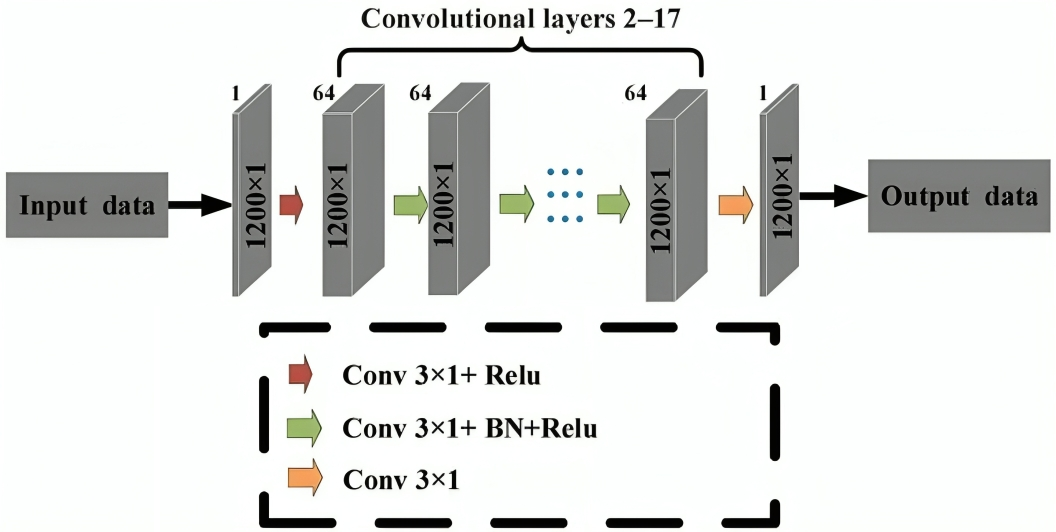
\includegraphics[scale=0.3]{../assets/dncnn.png}
    \captionsetup{justification=centering}
    \caption{Architettura di DnCNN \cite{dncnn_img}} \label{fig:dncnn}
\end{figure}

La rete è addestrata per apprendere la mappatura residua $R(I) = I - I_{\text{denoised}}$, dove $I$ è l'immagine rumorosa e $I_{\text{denoised}}$ è l'immagine a cui è stato rimosso il rumore. Durante l'inferenza, la nuova immagine si ottiene sottraendo il rumore stimato dall'immagine di input:

$$I_{\text{denoised}} = I - R(I)$$

Un modello pre-addestrato di DnCNN (DnCNN-S-25: con $\sigma$ = 25, e addestrato sul dataset \href{https://github.com/cszn/KAIR}{Train400} di Kai Zhang) è stato utilizzato per ridurre il rumore nelle immagini lunari, migliorando la qualità delle immagini e preparandole per il processo di stacking. La procedura utilizzata per la riduzione del rumore con DnCNN è riportata nell'\cref{alg:dncnn}.

\begin{algorithm}[H]
    \caption{\texttt{- Riduzione del rumore con DnCNN}:\\ Data un'immagine $I$, l'algoritmo restituisce l'immagine denoised $Out$.} \label{alg:dncnn}
    \begin{algorithmic}[1]
        \Function{denoise\_image}{$I$}
            \State $I_n \gets$ Normalizza $I$ tra $0$ e $1$ \Comment{Normalizzazione}
            \State $T \gets$ Converti $I_n$ in tensore
            \State $M \gets$ Carica il modello pre-addestrato DnCNN
            \State $N \gets M(T)$ \Comment{Stima del rumore}
            \State $Out \gets I_n - N$ \Comment{Sottrazione del rumore}
            \State $Out \gets$ Denormalizza $Out$ al range originale
            \State \textbf{return} $Out$
        \EndFunction
    \end{algorithmic}
\end{algorithm}

\subsection{Unsharp Masking e personalizzazione} \label{subsec:unsharp_mask}

L'\textbf{Unsharp Masking} è una tecnica utilizzata per aumentare la nitidezza dei dettagli in un'immagine. Consiste nel sottrarre una versione sfocata dell'immagine originale dall'immagine stessa, enfatizzando i dettagli e i bordi \cite{unsharp_mask_book}. La procedura standard è la seguente:

\begin{algorithm}[H]
    \caption{\texttt{Unsharp Mask}:\\ Data un'immagine $I$, l'algoritmo restituisce l'immagine nitida $Out$.} \label{alg:unsharp}
    \begin{algorithmic}
        \Function {unsharp\_mask}{$I, \alpha$}
            \State $I_{\text{B}} \gets$ Gaussian\_Blur($I$) \Comment{Sfocatura}
            \State $M \gets I - I_{\text{B}}$ \Comment{Calcola la maschera}
            \State $Out \gets I + \alpha \cdot M$ \Comment{Amplifica i dettagli}
            \State \textbf{return} $Out$
        \EndFunction
    \end{algorithmic}
\end{algorithm}


L'Unsharp Masking è un metodo semplice ed efficace per migliorare la nitidezza delle immagini, ma può introdurre artefatti e rumore, specialmente se il fattore di forza $\alpha$ è troppo elevato. Per evitare questi problemi, è possibile personalizzare la procedura di Unsharp Masking, ad esempio applicando un filtro di sfocatura diverso, regolando il fattore di forza o utilizzando tecniche di \textit{edge-aware filtering} per preservare i dettagli \cite{unsharp_mask}.

In questo progetto è stata implementata una versione personalizzata dell'unsharp masking che combina la riduzione del rumore tramite DnCNN e l'uso di una maschera basata sul gradiente dell'immagine.

L'applicazione di DnCNN alle immaginni lunari ha portato a risultati a prima vista deludenti. Infatti, l'immagine risultante era molto più sfocata rispetto all'originale. Questo è dovuto al fatto che DnCNN è stato addestrato per rimuovere il rumore, ma non per preservare i dettagli. Per ovviare a questo problema, come riportato nell'\cref{alg:custom_unsharp}, è stata utilizzata una maschera basata sul gradiente dell'immagine originale, che enfatizza i dettagli e i bordi in sezioni dell'immagine con valori del gradiente maggiori, mentre applica una riduzione del rumore maggiore nelle zone più uniformi (con valori del gradiente minori).

\begin{algorithm} [H]
    \caption{\texttt{Unsharp Masking personalizzato}:\\ Data un'immagine $I$, un, l'algoritmo restituisce l'immagine nitida $Out$.} \label{alg:custom_unsharp}

    \begin{algorithmic}
        \Function{custom\_unsharp}{$I, \alpha, \beta, thr$}
            \State $I_{\text{D}} \gets$ \Call{denoise\_image}{$I$} \Comment{Riduzione del rumore con l'\cref{alg:dncnn}}
            \State $I_{\text{D}} \gets (I_{\text{D}} \times \alpha) + I \times (1-\alpha)$ \Comment{Attenuazione del denoising}
            \State $G \gets$ Gradient($I$) \Comment{Calcolo del gradiente}
            \State $D_{\text{M}} \gets$ Get\_Mask$(G, thr)$ \Comment{Maschera di denoising}
            \State $D_{\text{M}} \gets$ Gaussian\_Blur$(D_{\text{M}})$ \Comment{Sfoca leggermente la maschera}
            \State $S_{\text{M}} \gets 1-D_{\text{M}}$ \Comment{Maschera di sharpening}
            \State $D \gets (I - I_{\text{D}}) \times \beta$ \Comment{Estrazione dei dettagli}
            \State $Out \gets (I_{\text{D}} \times D_{\text{M}}) + (I + D)\times S_{\text{M}}$ \Comment{Unsharping con dettagli amplificati}
            \State \textbf{return} $Out$
        \EndFunction
    \end{algorithmic}
\end{algorithm}

dove $Get\_Mask(I, thr)$ è una funzione che restituisce una maschera $M$ tale che:

$$
M(i,j) = \begin{cases} 1 & \text{se } G(i,j) < thr \\ 0 & \text{altrimenti} \end{cases}
$$

Il processo consiste dunque in diversi passaggi fondamentali. Si inizia con la riduzione del rumore, applicando il modello DnCNN all'immagine originale per ottenere una versione con rumore ridotto ($I_{\text{D}}$).
Successivamente, si effettua un \textit{blend} delle immagini, combinando l'immagine denoised e quella originale con un fattore $\alpha$, per preservare parte dei dettagli originali.
Il passo successivo prevede il calcolo del gradiente ($G$) dell'immagine originale per individuare le aree con dettagli significativi.
A questo punto, vengono create delle maschere ($D_{\text{M}}$, $S_{\text{M}}$, rispettivamente \textit{Denoise Mask, Sharpen Mask}) basate sul gradiente per distinguere le zone un cui applicare maggior denoising o amplificare i dettagli.
Per l'amplificazione dei dettagli ($D$), si calcola la differenza tra l'immagine originale e quella denoised, amplificandola con un fattore $\beta$ nelle zone con dettagli significativi.
Infine, si combinano le immagini utilizzando le maschere, ottenendo un'immagine finale ($Out$) in cui i dettagli sono stati amplificati e il rumore ridotto.

\subsection{Rimozione dello sfondo}

Se il cielo negli scatti non è perfettamente uniforme, 
potrebbero essere presenti gradienti di luminosità o rumore che influenzano negativamente il processo di stacking. Per ovviare a questo problema, è possibile rimuovere lo sfondo dalle immagini, enfatizzando i dettagli e riducendo l'effetto di gradienti di luminosità.

Una tecnica molto semplice per rimuovere lo sfondo consiste nell'applicare una maschera all'immagine, mantenendo solo i pixel con intensità al di sotto di una soglia specificata. Questo metodo è efficace per rimuovere lo sfondo uniforme, ma potrebbe non funzionare correttamente se il cielo presenta gradienti di luminosità o rumore.

Per superare queste limitazioni, è possibile applicare una trasformazione non lineare all'immagine, che enfatizza i dettagli e riduce il rumore. In questo progetto è stata utilizzata una trasformazione logistica, che comprime i valori dei pixel in un intervallo limitato, enfatizzando i dettagli e riducendo il rumore. L'algoritmo per la rimozione dello sfondo con trasformazione logistica è riportato nell'\cref{alg:remove_background}.

\begin{algorithm}[H]
    \caption{\texttt{- Rimozione dello sfondo}:\\ Data un'immagine $I$ e i parametri $thr$ e $\alpha$, l'algoritmo restituisce l'immagine con lo sfondo rimosso $Out$.} \label{alg:remove_background}
    \begin{algorithmic}[1]
        \Function{remove\_background}{$I, thr, \alpha$}
            \State $M \gets I < thr$ \Comment{Calcola la maschera dello sfondo}
            \State $Out \gets I$
            \For{ogni pixel $p$ in $M$ dove $M[p]=\text{True}$} 
                \State $Out[p] \gets I[p] \times \dfrac{1}{1 + \exp(-\alpha \times (I[p] - thr))}$ \Comment{Trasformazione logistica}
            \EndFor
            \State \textbf{return} $Out$
        \EndFunction
    \end{algorithmic}
\end{algorithm}

\section{Stacking delle immagini} \label{sec:stacking}

Lo \textbf{stacking} è una tecnica fondamentale nell'astrofotografia che consiste nel combinare più immagini dello stesso soggetto per migliorare il rapporto segnale-rumore e rivelare dettagli altrimenti invisibili.

\subsection{Algoritmi di stacking} \label{subsec:stacking}

Questa tecnica sfrutta il fatto che il rumore è un processo stocastico, mentre il segnale è deterministico. Quando si combinano più immagini dello stesso soggetto, il segnale rimane costante, mentre il rumore si riduce proporzionalmente alla radice quadrata del numero di immagini combinate. Questo significa che, se si combinano $N$ immagini, il rapporto segnale-rumore migliora di un fattore $\sqrt{N}$ \cite{stacking}.

Esistono diversi metodi per combinare le immagini durante lo stacking. Nel progetto sono stati implementati quattro metodi di stacking:

\begin{itemize}
    \item \textbf{Mean}: calcola la media pixel per pixel delle immagini. Questo metodo è utile per ridurre il rumore gaussiano e migliorare la qualità dell'immagine finale.
    $$
    I_{stacked} = \dfrac{1}{N} \sum_{i=1}^{N} I_i
    $$
    \item \textbf{Median}: calcola il valore mediano pixel per pixel delle immagini. Questo metodo è utile per ridurre il rumore impulsivo e rimuovere gli outlier.
    $$
    I_{stacked} = \text{median}(I_1, I_2, \ldots, I_N)
    $$
    \item \textbf{Sigma clipping}: calcola la media pixel per pixel delle immagini, escludendo i pixel con valori al di fuori di un intervallo di soglia. Questo metodo è utile per ridurre l'effetto di outlier e artefatti.
    $$
    I_{stacked}(x,y) = \dfrac{1}{N} \sum_{i=1}^{N} I_i(x,y) \quad \text{dove} \quad |I_i(x,y) - \text{mean}(I(x,y))| < k \cdot \sigma(x,y)
    $$
    \item \textbf{Weighted mean}: calcola la media pesata pixel per pixel delle immagini, assegnando pesi diversi in base ad una metrica di qualità, come la nitidezza.
    $$
    I_{stacked} = \dfrac{\sum_{i=1}^{N} W_i \cdot I_i}{\sum_{i=1}^{N} W_i}
    $$
\end{itemize}

L'algoritmo che ha portato a risultati migliori è la media pesata, molto comune in astrofotografia \cite{stacking_algos}, in particolare pesati in base alla nitidezza dell'immagine. L'algoritmo per il calcolo della media pesata è riportato nell'\cref{alg:weighted_mean}.

\begin{algorithm}[H]
    \caption{\texttt{- Stacking con media pesata}:\\ Dato un insieme di immagini $I$ e i pesi $W$, l'algoritmo restituisce l'immagine combinata $Out$.} \label{alg:weighted_mean}
    \begin{algorithmic}[1]
        \Function{weighted\_mean}{$I, W$}
            \State $N \gets$ \text{numero di immagini in } $I$
            \State $H, W_{\text{sum}} \gets 0$
            \For{$i \gets 1$ to $N$}
                \State $H \gets H + W[i] \times I[i]$ \Comment{Somma pesata}
                \State $W_{\text{sum}} \gets W_{\text{sum}} + W[i]$ \Comment{Somma dei pesi}
            \EndFor
            \State $Out \gets H / W_{\text{sum}}$ \Comment{Normalizzazione}
            \State \textbf{return} $Out$
        \EndFunction
    \end{algorithmic}
\end{algorithm}

Questo metodo è particolarmente efficace quando si combinano immagini con differenti livelli di nitidezza, contrasto e rumore, perchè, con una piccola modifica, permette anche di scartare una percentuale di immagini con qualità inferiore, riducendo l'effetto di artefatti e outlier.

\section{Post-Processing delle immagini} \label{sec:postprocessing}

Il post-processing delle immagini è l'ultima fase dell'elaborazione delle immagini lunari, necessaria per migliorare la qualità dell'immagine finale e renderla pronta per l'analisi e la visualizzazione. Questa fase comprende principalmente la regolazione del contrasto e della luminosità, la rimozione di artefatti e la correzione del bilanciamento del colore. 

Questa fase viene generalmente svolta su programmi di editing professionali come photoshop o lightroom, ma è possibile automatizzare il processo utilizzando algoritmi di elaborazione delle immagini.

\subsection{Miglioramento di nitidezza e contrasto} \label{subsec:contrast}

Per quanto riguarda l'aumento della nitidezza, l'\hyperref{unsharp_mask}{Unsharp Masking} (tradizionale) rimane uno dei metodi più efficaci, in quanto enfatizza i dettagli e i bordi dell'immagine. Tuttavia, è importante regolare attentamente i parametri per evitare artefatti e rumore.

L'\textbf{equalizzazione dell'istogramma} è una tecnica che distribuisce uniformemente i valori dei pixel nell'intervallo dinamico dell'immagine, migliorando il contrasto e la luminosità. Tuttavia, l'equalizzaziome standard può amplificare il rumore in aree omogenee e ridurre i dettagli in aree con contrasto già elevato. Inoltre, se l'immagine ha un contrasto limitato, l'equalizzazione dell'istogramma può produrre un'immagine sovraesposta o sottoposta, generando artefatti e perdita di dettagli.

Per superare queste limitazioni, è stata utilizzata la tecnica \textbf{CLACHE} (Contrast Limited Adaptive Histogram Equalization). CLACHE suddivide l'immagine in piccole regioni chiamate \textit{tile} e applica l'equalizzazione dell'istogramma a ciascuna regione separatamente. Inoltre, limita il contrasto di ciascuna regione per evitare l'amplificazione del rumore e la sovraesposizione. L'algoritmo per l'equalizzazione dell'istogramma con CLACHE è riportato nell'\cref{alg:clache}.

\begin{algorithm}[H]
    \caption{\texttt{- Equalizzazione dell'istogramma con CLACHE}:\\ Data un'immagine $I$, l'algoritmo restituisce l'immagine equalizzata $Out$.} \label{alg:clache}
    \begin{algorithmic}
        \Function{enhance\_contrast}{$I, \text{clip\_limit}, \text{tile\_grid\_size}$}
            \State $I_{\text{CLAHE}} \gets$ \text{Inizializza un'immagine vuota}
            \State $I_{\text{LAB}} \gets$ Converti $I$ in spazio colore LAB
            \State $L, A, B \gets$ Estrai i canali L, A, B da $I_{\text{LAB}}$
            \State $C \gets$ \text{Inizializza un'oggetto} CLACHE \text{con} tile\_grid\_size \text{e} clip\_limit
            \State $L_{\text{CLAHE}} \gets C.apply\_CLAHE(L)$ \Comment{Applica CLACHE al canale L}
            \State $I_{\text{CLAHE}} \gets$ Combina $L_{\text{CLAHE}}$, $A$ e $B$ in un'immagine
            \State \textbf{return} $I_{\text{CLAHE}}$
        \EndFunction
    \end{algorithmic}
\end{algorithm}

Lo spazio LAB è un modello di colore che separa la luminosità ($L$) dal colore ($A$ e $B$), rendendo più semplice l'applicazione di tecniche di miglioramento del contrasto e della luminosità. L'equalizzazione dell'istogramma viene applicata solo al canale $L$, che rappresenta la luminosità dell'immagine, mentre i canali $A$ e $B$ rimangono inalterati. Questo permette di migliorare il contrasto e la luminosità dell'immagine senza influenzare il colore.

Tramite \texttt{clip\_limit} e \texttt{tile\_grid\_size} è possibile regolare il contrasto e la dimensione delle regioni su cui applicare l'equalizzazione dell'istogramma. Un \texttt{clip\_limit} più alto aumenta il contrasto, mentre un \texttt{tile\_grid\_size} più piccolo permette di equalizzare dettagli più fini.

\subsection{Bilanciamento del colore} \label{subsec:color_balance}

Nel contesto dell'astrofotografia lunare, il bilanciamento del colore è generalmente meno critico rispetto ad altre forme di fotografia, poiché la luna appare prevalentemente in toni di grigio. Tuttavia, può essere utile per correggere tonalità dell'immagine e migliorare la qualità visiva, evidenziando lievi variazioni cromatiche dovute alla composizione minerale sulla superficie. Esistono diversi metodi per il bilanciamento del colore:

\begin{itemize}
    \item \textbf{Correzione automatica del bilanciamento del bianco}: utilizza algoritmi di bilanciamento del bianco automatici per correggere il colore dell'immagine in base alla temperatura del colore. Questo metodo è utile per correggere il colore in modo rapido e semplice.
    \item \textbf{Correzione manuale del bilanciamento del bianco}: permette di regolare manualmente il bilanciamento del bianco dell'immagine, selezionando un punto neutro o una zona grigia come riferimento. Questo metodo è utile per ottenere un controllo preciso sul colore dell'immagine.
    \item \textbf{Correzione del colore selettiva}: permette di regolare selettivamente i toni, la saturazione e la luminosità di specifici colori nell'immagine. Questo metodo è utile per migliorare il colore e il contrasto di parti specifiche dell'immagine.
\end{itemize}

Per questo progetto, è stato adottato un metodo di bilanciamento del colore automatico basato sull'assunzione delle \textbf{Shades of Gray} (tonalità di grigio). Questo approccio presuppone che l'immagine abbia una distribuzione equilibrata delle tonalità di grigio, permettendo di correggere le deviazioni cromatiche tramite la normalizzazione dei canali di colore \cite{shades_of_gray}. I passaggi principali sono i seguenti:

\begin{enumerate}
    \item \textbf{Calcolo della media normalizzata per ciascun canale}: Per ogni canale di colore (RGB), si calcola la media dei valori dei pixel elevati a una potenza specificata ($p$). Questa operazione enfatizza i valori più alti, riducendo l'influenza dei pixel più scuri.
    $$
    S[c] = \left(\dfrac{1}{M \times N} \sum_{x=1}^{M} \sum_{y=1}^{N} I(x,y,c)^{p} \right)^{1/p}
    $$
    \item \textbf{Calcolo della media delle \texttt{norm\_values}}: Si calcola la media delle medie normalizzate ottenute per ciascun canale. Questo valore rappresenta il target di normalizzazione per ogni canale.

    $$
    \mu = \dfrac{1}{3} \sum_{c=1}^{3} S[c]
    $$

    \item \textbf{Calcolo dei fattori di scala}: Per ogni canale, si determina un fattore di scala che normalizza la media del canale rispetto alla media complessiva. Questo assicura che ciascun canale contribuisca equamente alla tonalità di grigio finale.
    
    $$
    f[c] = \dfrac{\mu}{S[c]}
    $$
    
    \item \textbf{Applicazione dei fattori di scala}: Si moltiplicano i valori dei pixel di ogni canale per il rispettivo fattore di scala, correggendo le deviazioni cromatiche.
    
    $$
    Out(x,y,c) = I(x,y,c) \times f[c]
    $$
    
    \item \textbf{Clipping dei valori}: Infine, si assicura che i valori dei pixel rimangano nel range $[0, 1]$ per evitare distorsioni cromatiche.
    
    $$
    Out = \text{clip}(Out, 0, 1)
    $$

\end{enumerate}


Questa tecnica garantisce che l'immagine risultante abbia una distribuzione equilibrata delle tonalità di grigio, correggendo automaticamente le deviazioni cromatiche senza richiedere interventi manuali.
Lo pseudocodice che racchiude questi passaggi è riportato nell'\cref{alg:shades_of_gray}.

\begin{algorithm}[H]
    \caption{\texttt{- Shades of Gray - bilanciamento del colore}:\\ Data un'immagine $I$, l'algoritmo restituisce l'immagine bilanciata $Out$.} \label{alg:shades_of_gray}
    \begin{algorithmic}[1]
        \Function{shades\_of\_gray}{$I, p=6$}
            \State $M, N \gets$ dimensioni di $I$
            \State $S \gets$ inizializza vettore per le norme
            \For{$c \gets 1$ to $3$} \Comment{Per ogni canale RGB}
                \State $S[c] \gets \left(\dfrac{1}{M \times N} \sum_{x=1}^{M} \sum_{y=1}^{N} I(x,y,c)^p \right)^{1/p}$ 
            \EndFor
            \State $\mu \gets \dfrac{1}{3} \sum_{c=1}^{3} S[c]$ \Comment{Media delle norme}
            \For{$c \gets 1$ to $3$}
                \State $f[c] \gets \mu / S[c]$ \Comment{Fattori di scala}
                \For{$x \gets 1$ to $M$}
                    \For{$y \gets 1$ to $N$}
                        \State $Out(x,y,c) \gets I(x,y,c) \times f[c]$ \Comment{Applica bilanciamento}
                    \EndFor
                \EndFor
            \EndFor
            \State $Out \gets \text{clip}(Out, 0, 1)$ \Comment{Limita valori tra 0 e 1}
            \State \textbf{return} $Out$
        \EndFunction
    \end{algorithmic}
\end{algorithm}

\cleardoublepage